\documentclass[a4paper]{article}

%use the english line for english reports
%usepackage[english]{babel}
\usepackage[portuguese]{babel}
\usepackage[utf8]{inputenc}
\usepackage{indentfirst}
\usepackage{graphicx}
\usepackage{verbatim}


\begin{document}

\setlength{\textwidth}{16cm}
\setlength{\textheight}{22cm}

\title{\Huge\textbf{MOD X}\linebreak\linebreak\linebreak
\Large\textbf{Relatório Intercalar}\linebreak\linebreak
\linebreak\linebreak

\includegraphics[scale=0.1]{./images/feup-logo.png}\linebreak\linebreak
\linebreak\linebreak
\Large{Mestrado Integrado em Engenharia Informática e Computação} \linebreak\linebreak
\Large{Programação em Lógica}\linebreak
}

\author{\textbf{Grupo ModX3:}\\
António Manuel Vieira Ramadas - 201303568 \\
Rui Miguel Teixeira Vilares - 201207046 \\
\linebreak\linebreak \\
 \\ Faculdade de Engenharia da Universidade do Porto \\ Rua Roberto Frias, s\/n, 4200-465 Porto, Portugal \linebreak\linebreak\linebreak
\linebreak\linebreak\vspace{1cm}}

\maketitle
\thispagestyle{empty}

%************************************************************************************************
%************************************************************************************************

\newpage

%Todas as figuras devem ser referidas no texto. %\ref{fig:codigoFigura}
%
%%Exemplo de código para inserção de figuras
%%\begin{figure}[h!]
%%\begin{center}
%%escolher entre uma das seguintes três linhas:
%%\includegraphics[height=20cm,width=15cm]{path relativo da imagem}
%%\includegraphics[scale=0.5]{path relativo da imagem}
%%\includegraphics{path relativo da imagem}
%%\caption{legenda da figura}
%%\label{fig:codigoFigura}
%%\end{center}
%%\end{figure}
%
%
%\textit{Para escrever em itálico}
%\textbf{Para escrever em negrito}
%Para escrever em letra normal
%``Para escrever texto entre aspas''
%
%Para fazer parágrafo, deixar uma linha em branco.
%
%Como fazer bullet points:
%\begin{itemize}
	%\item Item1
	%\item Item2
%\end{itemize}
%
%Como enumerar itens:
%\begin{enumerate}
	%\item Item 1
	%\item Item 2
%\end{enumerate}
%
%\begin{quote}``Isto é uma citação''\end{quote}


%%%%%%%%%%%%%%%%%%%%%%%%%%
\section{O Jogo MOD X}

O MOD X é um jogo de tabuleiro, nascido em 2015, recomendado para jogadores com mais de 15 anos de idade.
Cada partida reúne 2 a 4 jogadores e tem a duração prevista de 20 a 30 minutos. 

\vspace{0.5cm}

\textbf{Componentes do jogo:}
\begin{itemize}
	\item 1 Tabuleiro 8x8;
	\item 56 peças de jogo em formato X (14 em cada cor);
	\item 72 marcadores de pontuação (18 em cada cor);
	\item 5 peças Joker em formato X (brancas);
\end{itemize}

\vspace{0.5cm}

\textbf{Objetivo do jogo:}

Conseguir formar o maior número de padrões possível, de forma a conseguir a melhor pontuação. O vencedor é o jogador com mais pontos.  

\vspace{0.5cm}

\begin{figure}[h!]
	\begin{center}
		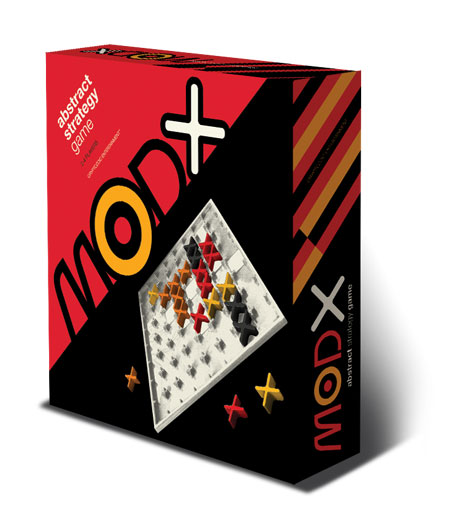
\includegraphics[scale=0.4]{./images/modx_box.jpg}
		\caption{Caixa do MOD X}
		\label{fig:1}
	\end{center}
\end{figure}

\vspace{0.5cm}

O MOD X é um jogo de tabuleiro de estratégia é divertido e fácil de aprender. 
O objetivo deste jogo é criar padrões com peças coloridas (vermelho, preto, amarelo e laranja) \footnote{https://boardgamegeek.com/boardgame/131387/mod-x}.

Cada jogador inicia o jogo com 14 peças e 18 marcadores.
Inicialmente, define-se a ordem dos jogadores e escolha das peças por parte dos jogadores.  
No seu turno, um jogador coloca uma peça no tabuleiro, com o objetivo de criar padrões específicos, que se traduzem em pontos.
Os padrões utilizados para ganhar pontos são o ''X'', o ''+'' e o ''cinco em linha''.

Existem umas peças de cor branca, dispostas inicialmente de forma aleatória, chamadas Jokers. O jogador pode usar essas peças para formar padrões, como se tratassem das suas próprias peças.

É suposto bloquear os adversários de modo que não consigam construir esses padrões\footnote{https://www.cryptozoic.com/games/mod-x}.

\vspace{0.5cm}

\begin{figure}[h!]
	\begin{center}
		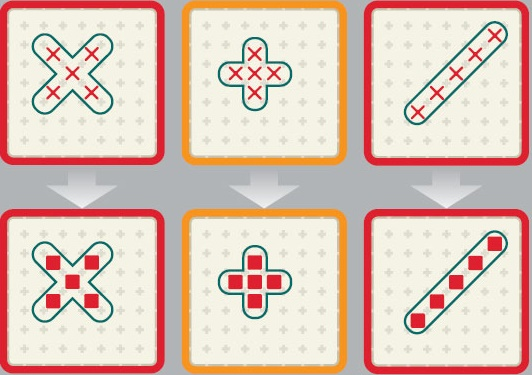
\includegraphics[scale=0.4]{./images/modx_score.jpg}
		\caption{Padrões usados}
		\label{fig:2}
	\end{center}
\end{figure}

\vspace{0.5cm}

No final, o primeiro jogador a atingir um certo número de pontos, determinado inicialmente pelo número de jogadores, é o vencedor.
O jogo pode também terminar quando um jogador terminar com as suas peças ou marcadores.
Nesse caso, o jogo termina imediatamente e ganha o jogador com mais pontos até ao momento.


%%%%%%%%%%%%%%%%%%%%%%%%%%
\section{Representação do Estado do Jogo}

Descrever a forma de representação do estado do tabuleiro (tipicamente uma lista de listas), com exemplificação em Prolog de posições iniciais do jogo, posições intermédias e finais, acompanhadas de imagens ilustrativas.


%%%%%%%%%%%%%%%%%%%%%%%%%%
\section{Visualização do Tabuleiro}

Descrever a forma de visualização do tabuleiro em modo de texto e o(s) predicado(s) Prolog construídos para o efeito.
Deve ser incluída pelo menos uma imagem correspondente ao output produzido pelo predicado de visualização.


%%%%%%%%%%%%%%%%%%%%%%%%%%
\section{Movimentos}

Elencar os movimentos (tipos de jogadas) possíveis e definir os cabeçalhos dos predicados que serão utilizados (ainda não precisam de estar implementados).


\end{document}
